This task focused on predicting Vietnamese gold prices using a linear regression model implemented in PySpark.
The objective was to transform historical time-series data into a suitable format for regression,
train a model, and evaluate its predictive performance.

\subsection{Overview of Linear Regression (LR)}
\label{subsec:overview-of-linear-regression}

LR is a supervised learning algorithm that models the linear relationship between a continuous target variable ($y$) and one or more independent predictor variables (features $\mathbf{x}$). The goal is to find an optimal linear function that best predicts $y$ given $\mathbf{x}$.

For a single feature $x$, the model is:
\begin{equation}
    y = \beta_0 + \beta_1 x + \epsilon
    \label{eq:simple_lr}
\end{equation}
With multiple features $x_1, x_2, \ldots, x_p$, it extends to:
\begin{equation}
    y = \beta_0 + \beta_1 x_1 + \beta_2 x_2 + \ldots + \beta_p x_p + \epsilon
    \label{eq:multiple_lr}
\end{equation}
where $\beta_0$ is the intercept, $\beta_j$ are the feature coefficients (weights), and $\epsilon$ is the error term.
The coefficients are typically learned by minimizing a loss function, such as Mean SquaredError (MSE), often using optimization algorithms like L-BFGS. Key assumptions include linearity, independence of errors, and homoscedasticity.
This project applies LR to predict gold prices based on historical price features.

\subsection{Data Preparation}
\label{subsec:data-preparation}
\begin{itemize}
    \item \textbf{Dataset:} The primary data source was \texttt{gold\_prices.csv} (2009/08/01 to 2025/01/01),
    read into a PySpark DataFrame.
    \item \textbf{Feature Engineering:} For each target date $t$, features were the respective `Buy Price' or `Sell Price' values from the 10 consecutive preceding days.
    PySpark's \texttt{Window} functions and \texttt{lag} operation were used, followed by \texttt{VectorAssembler} to create feature vectors (e.g., \texttt{Previous Buy Price(s)}). 4000 samples were generated (\texttt{random\_state=38}).
    \item \textbf{Data Splitting:} The generated DataFrame was randomly split into training (70\%) and testing (30\%) sets (\texttt{seed=2}).
\end{itemize}

\subsection{Model Implementation and Training}
\label{subsec:model-implementation-and-training}

Two separate Linear Regression models (\texttt{pyspark.ml.regression.LinearRegression}) were developed: one for `Buy Price' and one for `Sell Price', using their respective 10-day historical price vectors as features and the current price as the label.
Models were configured with the \texttt{`l-bfgs'} solver and trained on the 70\% training subset.

\subsection{Experimental Results and Evaluation}
\label{subsec:experimental-results-and-evaluation}

\subsubsection{Overall Results}\text{}

The performance of the trained models was evaluated on both training and testing sets.
The R$^2$ values (consistently $>$ 0.999), low RMSE/MAE, and high Explained Variance scores indicate strong predictive accuracy and good generalization to unseen data, with no significant overfitting observed.

\smallskip

\subsubsection{Loss History During Training}\text{}

%Line chart (Fig.~\ref{fig:buy_price_model_loss}) illustrated the objective function value per iteration, showing rapid convergence for both `Buy Price' and `Sell Price' model.

\begin{figure}[H]
    \centering
    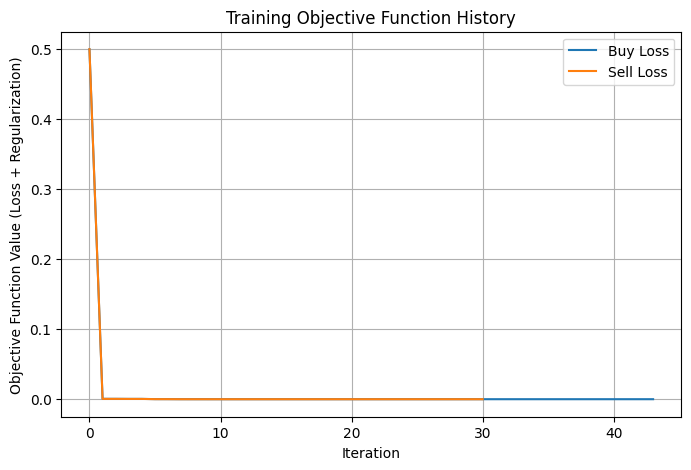
\includegraphics[width=0.8\linewidth]{images/loss_history}
    \caption{Loss History of Buy Price Prediction Model}
    \label{fig:buy_price_model_loss}
\end{figure}

\subsubsection{Performance Comparison}\text{}

%Bar charts (Fig.~\ref{fig:rmse_r2_mae} nd Fig.~\ref{fig:train_test_var}) contrasted evaluation metrics (RMSE, R$^2$, MAE, Explained Variance) between training and testing sets, visually confirming robust generalization.

\begin{figure}[H]
    \centering
    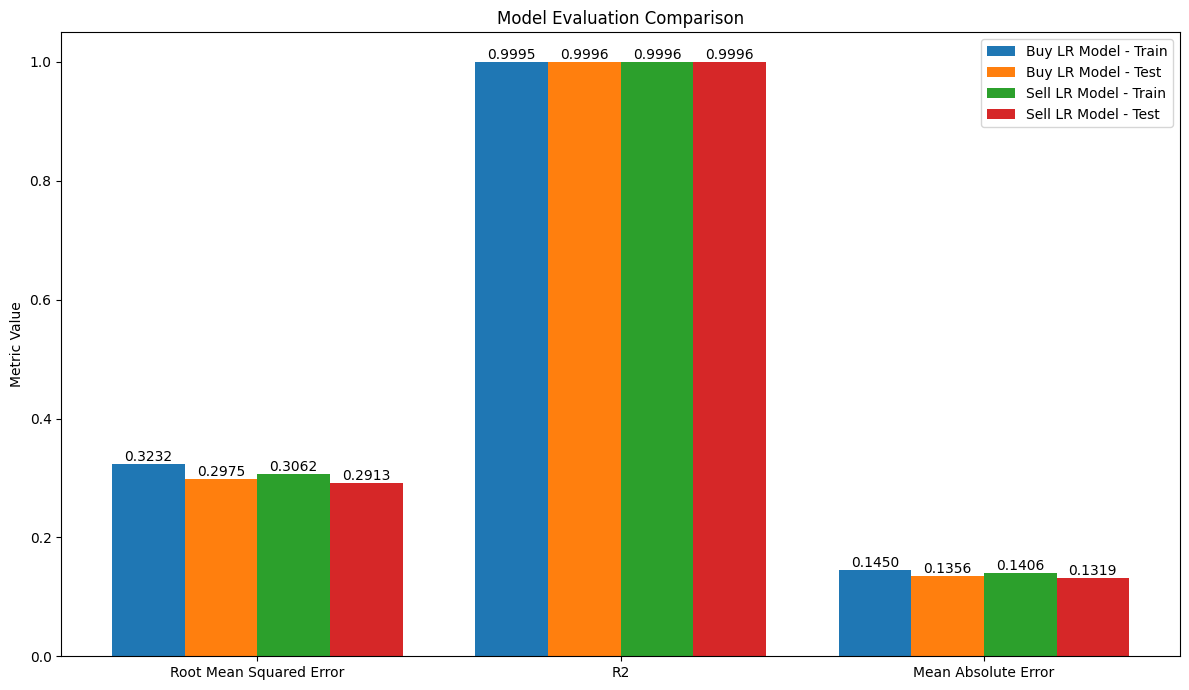
\includegraphics[width=0.8\linewidth]{images/rmse_r2_mae}
    \caption{'Buy Price' and 'Sell Price' Models Performance.}
    \label{fig:rmse_r2_mae}
\end{figure}

\begin{figure}[H]
    \centering
    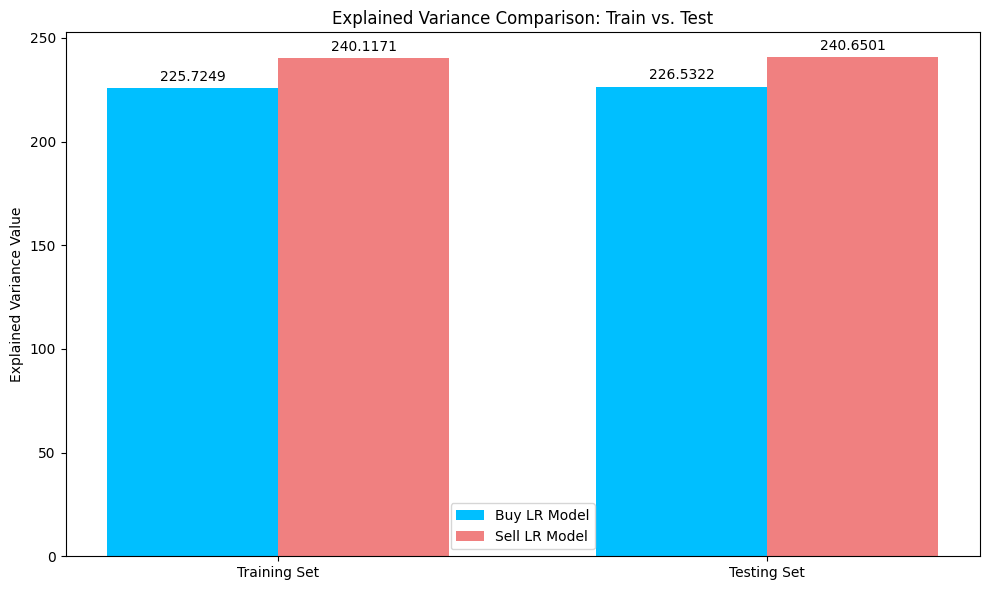
\includegraphics[width=0.8\linewidth]{images/train_test_var}
    \caption{'Buy Price' and 'Sell Price' Models Explained Variance Performance.}
    \label{fig:train_test_var}
\end{figure}